\documentclass[10pt,a4paper,twocolumn,twoside]{article}
\usepackage[utf8]{inputenc}
\usepackage[catalan]{babel}
\usepackage{multicol}
\usepackage{graphicx}
\usepackage{fancyhdr}
\usepackage{times}
\usepackage{titlesec}
\usepackage{url}
\usepackage{multirow}
\usepackage{lettrine}
\usepackage[top=2cm, bottom=1.5cm, left=2cm, right=2cm]{geometry}
\usepackage[figurename=Fig.,tablename=TAULA]{caption}
\captionsetup[table]{textfont=sc}

\author{\LARGE\sffamily Miquel Freixes Faya}
\title{\Huge{\sffamily Anàlisis de la relació entre les emisions de Co2 i l'augment de la temperatura, mitjançant tècniques i tecnologies de Big Data. Informe Inicial}}
\date{}

\newcommand\blfootnote[1]{%
  \begingroup
  \renewcommand\thefootnote{}\footnote{#1}%
  \addtocounter{footnote}{-1}%
  \endgroup
}

%
%\large\bfseries\sffamily
\titleformat{\section}
{\large\sffamily\scshape\bfseries}
{\textbf{\thesection}}{1em}{}

\begin{document}

\fancyhead[LO]{\scriptsize MIQUEL FREIXES FAYA: TÍTOL DEL TREBALL}
\fancyhead[RO]{\thepage}
\fancyhead[LE]{\thepage}
\fancyhead[RE]{\scriptsize EE/UAB TFG INFORMÀTICA: TÍTOL (ABREUJAT SI ÉS MOLT LLARG)}

\fancyfoot[CO,CE]{}

\fancypagestyle{primerapagina}
{
   \fancyhf{}
   \fancyhead[L]{\scriptsize TFG EN ENGINYERIA INFORMÀTICA, ESCOLA D'ENGINYERIA (EE), UNIVERSITAT AUTÒNOMA DE BARCELONA (UAB)}
   \fancyfoot[C]{\scriptsize ``Febrer'' de 2019, Escola d'Enginyeria (UAB)}
}

%\lhead{\thepage}
%\chead{}
%\rhead{\tiny EE/UAB TFG INFORMÀTICA: TÍTOL (ABREUJAT SI ÉS MOLT LLARG)}
%\lhead{ EE/UAB \thepage}
%\lfoot{}
%\cfoot{\tiny{February 2015, Escola d'Enginyeria (UAB)}}
%\rfoot{}
\renewcommand{\headrulewidth}{0pt}
\renewcommand{\footrulewidth}{0pt}
\pagestyle{fancy}

%\thispagestyle{myheadings}
\twocolumn[\begin{@twocolumnfalse}

%\vspace*{-1cm}{\scriptsize TFG EN ENGINYERIA INFORMÀTICA, ESCOLA D'ENGINYERIA (EE), UNIVERSITAT AUTÒNOMA DE BARCELONA (UAB)}

\maketitle

\thispagestyle{primerapagina}
%\twocolumn[\begin{@twocolumnfalse}
%\maketitle
%\begin{abstract}
\begin{center}

{\vrule depth 0pt height 0.5pt width 4cm\hspace{7.5pt}%
\raisebox{-3.5pt}{\fontfamily{pzd}\fontencoding{U}\fontseries{m}\fontshape{n}\fontsize{11}{12}\selectfont\char70}%
\hspace{7.5pt}\vrule depth 0pt height 0.5pt width 4cm\relax}

\end{center}

\bigskip
%\end{abstract}
\end{@twocolumnfalse}]

\blfootnote{$\bullet$ E-mail de contacte: m.freixes.faya@gmail.com}
\blfootnote{$\bullet$ Menció realitzada: Tecnologies de la Informació}
\blfootnote{$\bullet$ Treball tutoritzat per: Jordi Casas Roma (departament)}
\blfootnote{$\bullet$ Curs 2018/19}

\section{Objectius}
\lettrine[lines=3]{L}{'objectiu} principal d'aquest treball és analitzar com ha augmentat la temperatura a la superfície terrestre al llarg dels anys. No obstant això, també es vol comparar aquestes temperatures amb altres dos paràmetres, per veure quina implicació tenen en l'augment. També es pot donar el cas que no es trobi cap relació entre aquests tres volums de dades. Concretament els dos volums de dades que s'analitzaran són:
\begin{itemize}
\item La quantitat de Co2 que ha produït cada país al llarg d’un any sencer. [1]
\item La petjada ecològica mitjana de cada país al llarg de cada any. [2] Això és una forma de representar l'àrea de vegetació i/o aigua que es necessita per satisfer les necessitats d'una persona durant un any. [3] El conjunt de dades escollit agafarà una mitjana de totes les persones de cada país.   
\end{itemize}

Aquests objectius van enfocats a aprendre a processar diferents Datasets, aconseguint un que estigui destinat a entrenar un algorisme de Machine Learning. Aquest algorisme ha d'acabar sent capaç de predir les tendències en la temperatura a cada país. Per tant, un altre objectiu serà entendre com es pot entrenar un algorisme i extreure els resultats que pugui treure. Com a objectiu addicional es vol fer aquest anàlisis amb diversos algorismes per poder fer una comparativa de l'efectivitat i ràtio d'encert de cada un d'ells.

\section{Planificació}
Tal com es mostra en el diagrama de Gantt de la Figura 1, aquest TFG té diverses fases bastant ben diferenciades. Aquestes són:
\begin{itemize}
\item Una primera fase de recerca: Aquí cal investigar si s'han fet treballs semblants al del TFG, ja sigui sobre el canvi climàtic, sobre processament de datasets. També cal fer una recerca sobre quins algorismes de Machine Learning caldrà entrenar i com entrenar-los, a causa del gran nombre d'algorismes existents. Cal mirar l'estat de l'art, a més d'aprofitar-lo per aprendre les millors tècniques a aplicar i com aplicar-les als datasets escollits.

\item La segona va destinada al processament dels Datasets. Tot i que els datasets escollits tenen les dades netejades, cada un té columnes diferents i fins i tot algun dataset té dades de períodes temporals que altres no tenen. La idea bàsica és seleccionar les columnes i files més rellevants per la investigació que es vol fer i solucionar algun problema en la compatibilitat de les dades. Un exemple de problema a solucionar ve donat pel Dataset de les temperatures. Aquest Dataset et diu les temperatures mitjanes al llarg dels anys de moltes ciutats arreu del món, però no dels països. En canvi els altres dos datasets tracten de les emissions en cada país i no de les ciutats. En acabar es tindrà un únic dataset amb les dades més rellevants en un període de temps determinat, en principi es vol agafar les dades entre l'any 1990 i el 2013.

\item La tercera agafa el dataset resultant de la fase anterior i l'utilitza per entrenar un algorisme de Machine Learning. Aquest algorisme s'escollirà al llarg de la primera i segona fase segons els tipus de dades que s'acabin analitzant. No es destinarà el 100\% del dataset pel fet que es reservarà una part per comprovar si l'algorisme funciona correctament. Concretament es té pensat destinar un 80\% a l'entrenament i un 20\%  per les comprovacions posteriors.

\item La quarta fase acabarà sent la representació dels resultats que s'hauran extret de l'algorisme, ja sigui a partir de gràfics estadístics, diagrames o gràfics lineals. També es farà una reflexió sobre el bon o mal funcionament de l'algorisme i es trauran conclusions.

\item Hi ha una última fase que només es farà si hi ha suficient temps. Aquesta consistirà a repetir la tercera i la quarta amb diferents algorismes i després comparar els resultats que extreu cada un. Posteriorment es farà una anàlisi de les característiques de cada un com l'eficiència, la dificultat d'entrenar-lo o el percentatge d'error de cada un.

\end{itemize}
Totes aquestes fases s'aniran documentant per tal d'anar fent l'informe final i com es pot veure en el diagrama es té pensat deixar bastant de temps per poder acabar l'informe i/o tenir marge per si apareixen situacions inesperades o complicacions.

\section{Metodologia}
A l'hora de fer projectes hi ha un gran nombre de metodologies per escollir, però en l'àmbit de la informàtica les més utilitzades són les Agile. Això és degut a l'increment del nombre de projectes àgils acabats en èxit, respecte dels projectes on s'han aplicat les metodologies tradicionals. [2] Dins de la metodologia àgil hi ha diverses metodologies com Scrum, Kanban, XP... En aquest treball se seguirà la Kanban, a causa del fet que la metodologia Scrum no es podria aprofitar al màxim amb només una persona en el projecte. La principal raó per no escollir Scrum ha estat que molts papers els hauria de fer la mateixa persona, com el de Scrum Master, Product Owner... Algunes de les principals característiques no tindrien sentit. [3]

Kanban es basa en una taula de progrés on es fiquen les tasques per fer, les que s'estan fent i les fetes. Això permetrà un seguiment constant de com avança el projecte. També permet treballar segons prioritats, no per temps, i això s'ajusta molt bé al tipus de projecte que es desenvoluparà. Degut al fet que el projecte està format per tasques que es poden paral·lelitzar, i d'altres que no es poden fer sense una prèvia, apareixeran prioritats al llarg del desenvolupament. [4]

La fase del projecte destinada a l'anàlisi dels datasets es farà utilitzant el software d'Apache Spark a partir de Databricks. S'ha escollit Databricks perquè ofereix un petit clúster amb 6Gb de Ram gratuïtament per estudiants, uns recursos més que suficients per processar el volum de dades desitjat.
A part d'això, tot el progrés de cada etapa s'anirà guardant en un Git per tal de no perdre res i poder mantenir un històric dels canvis. En el Git es guardarà els informes, els codis i algorismes necessaris i els datasets amb les dades.
Per acabar, els codis es faran en el llenguatge de Python. Aquest llenguatge és molt utilitzat a l'hora de treballar amb algorismes de Machine Learning. A més, s'utilitzaran algorismes de la pàgina web de Scikit Learn, a causa de la gran varietat d'algorismes que ofereix i a la facilitat d'implementar-los. [8] 


\begin{thebibliography}{11}
\bibitem{1}
\url{https://www.kaggle.com/unitednations/international-greenhouse-gas-emissions}
\bibitem{2}
\url{https://www.kaggle.com/footprintnetwork/national-footprint-accounts-2018}

\bibitem{3}
"Ecological Footprint", \textit{WWF}. [En línia]. Disponible a: \url{https://wwf.panda.org/knowledge_hub/teacher_resources/webfieldtrips/ecological_balance/eco_footprint/}. [Accedit Octubre 4, 2018].
 
\bibitem{4}
"Sample Research", \textit{The Standish Group}.~[En~línia].~Disponible~a:~\url{https://www.standishgroup.com/sample_research}~[Accedit~Octubre~4,~2018].

\bibitem{5}
"Scrum Reference Card now available in English and Spanish",  \textit{Agile Methodology}. [En línia]. Disponible a: \url{http://agilemethodology.org/ }. [Accedit Octubre 4, 2018].

\bibitem{6}
"The Complete Guide to Understanding Agile Testing", \textit{QA Symphony}. [En línia].Disponible a: \url{https://www.qasymphony.com/blog/agile-methodology-guide-agile-testing/}. [Accedit Octubre 4, 2018].

\bibitem{7}
A.Géron, \textit{Hands-On Machine Learning with Scikit-Learn \& TensorFlow}. Sebastopol, CA: O’Reilly Media, 2017.

\bibitem{8}
"Supervised Learning", \textit{Scikit-Learn}. Disponible a: \url{http://scikit-learn.org/stable/supervised_learning.html#supervised-learning}. [Accedit Octubre 5, 2018].
\end{thebibliography}
\clearpage
\section{Annex}

\begin{figure}[!h]
\centering
	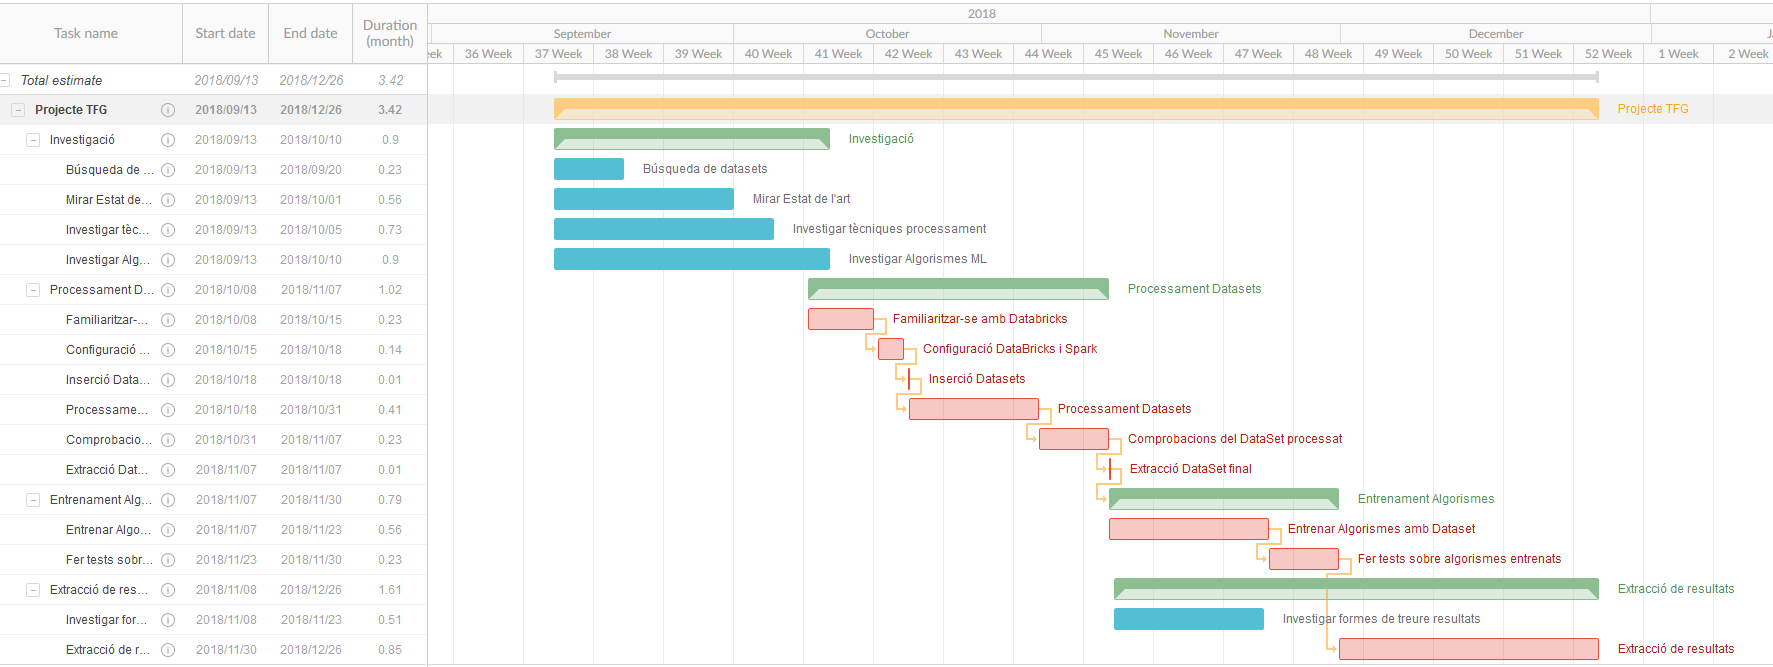
\includegraphics[width=1\textwidth]{img/diagrama_Gantt}

	\caption{Diagrama de Gantt}
	\label{fig-Gantt}
\end{figure}


\end{document}

